\title{Psychology Assignment}
\author{Name}
\documentclass{report}
\usepackage{graphicx}
\usepackage{appendix}
\usepackage{mathtools}
\graphicspath{ {Pictures/} }
\begin{document}
\maketitle
\tableofcontents
\chapter{Introduction}
Social psychology is the study of individual’s psychology in a group setting,  how the group may affect the individual and where certain traits within social interaction come from Conformity is where one individual is pressured into changing their actions or beliefs based on the effect a group has on them. Normative influence stems from the desire to be “normal”, and will often be affected by the group norms of the influencing party, and informational influence stems from a genuine belief that others will know more about the task at hand than they will, and therefore they look to them for guidance, so that the individuals desire to be “correct” is sated. One common factor which affects conformity is the size of the influencing party. Typically, larger groups will incite more conformity, as individuals believe a large majority to be correct. Another factor which could affect the conformity is similarity. If the individuals within the group are similar in other areas, they will be more likely to look to each other when undergoing an unknown task.

\section{Background Research}

\subsection{Jenness(1932)}
\subsubsection{Aim}
To find whether or not people will conform due to informational influence
\subsubsection{Method}
Jenness (1932) gave participants a jar of beans, and asked them to estimate how many beans are in the jar. He then grouped participants together and allowed them to discuss their answers, then asked them to guess again. This was in order to allow the majority to influence the individual.
\subsubsection{Results/Analysis}
Jenness found that most participants changed their answer to conform to the majority. These results show that, when given an ambiguous task, people will look upon others to inform their own answer.  This is therefore a landmark study into informational conformity, as the participants believed that the answer of the group was more likely to be correct than their own individual answer.
\subsection{Asch (1951)}
\subsubsection{Aim}
In 1951, Solomon Asch carried out a study on the effects of social pressure from a majority, and whether it could cause someone to conform.
\subsubsection{Method}
Asch gathered 50 male students in America, to carry out the task of judging the lengths of line. They would be shown a “target line” and three “comparison lines”. The participant had to guess what comparison line was closest to the target line. The participant was placed in a room with seven confederates, who had already decided on their answers before the task. The participant was not aware that the other people in the room were confederates, and believed that they were all genuine participants. The person had to state out loud which comparison line they believed to be the correct answer, but the true participant would always go last or second to last. There were 18 trials held, with 12 of them where the confederates decided to lie about the length of line.
\subsubsection{Results/Analysis}
Asch found that 32\% of the participants conformed to the answer of the confederates, even if it was clearly incorrect. 75\% of participants conformed at least one time, and 25\% of participants did not conform once. This is a landmark study into normative conformity as it shows that the people didn’t actually believe that the answer they were choosing is correct, but they went along with the majority anyway. This study is biased as the sample only compares across American male college students. Therefore this study is difficult to generalise. This study also has low ecological validity as it is a very artificial task that people are unlikely to be asked about in daily life.
\chapter{Study of Informational Conformity with an unknown majority (2018)}
\section {Aim}
The aim of this study was to determine whether or not an individual would conform to a group majority, even if they cannot directly see the majority themselves.
\section{Hypothesis}
The individual will conform to the majority, even if they do not know who the influencing party is directly.
\section {Method}
\subsection{Design}
The study was conducted in a lab environment, with an experimental format.
\subsection{Research of Extraneous or Confounding Variables}
The student’s intelligence level could have interfered with the task, as they would be able to judge the task better. The students’ personality and individual independence could have also affected the results of the experiment.
\subsection{Sampling Method and participants}
The participants involved were opportunity sampled. There were 24 participants taking part in total. The participants were all aged between 15 and 18, in high school education. Two people in the class were not able to take part due to the fact that they were already aware of the task at hand. There were 14 males and 10 females.
\subsection{Procedure}
Upon entering the class, the students were briefed. They were not able to be informed about the exact task at hand as that would confound results. They were told that they were to guess how many pieces of pasta were in a jar. They were shown the jar, and subsequently given “guess sheets”. Half of these guess sheets had falsified previous guesses already written on them by researchers, and half were blank. This was in order to determine whether or not the results would show a higher level of conformity on the sheets with previous answers
\begin{center}
\end{center}
\subsection{Materials needed}
\begin{itemize}
  \item One transparrent 50g bag of Tesco's own fusilli pasta
  \item Documents that must be signed in order to ensure informed consent
  \item Two sets of othewise identical "guess sheets", half of which would contain falsified "previous guesses"
\end{itemize}
\section{results}
\textit{All raw data can be found in the appendix section}
\subsection{Statistics to analyse results data}
There were a number of calculations performed on the raw data. These include:
\begin{itemize}
\item Finding the mean. In condition 1 (with “previous guesses”) this was found to be 358. In condition 2 (without “previous guesses”) the mean was 441. The false guesses averaged at 527. The mean was calculated by finding the sum of all the guesses and then divided it by the number of guesses in total.
\begin{displaymath}
M_1 = \frac{7+210+300+302+311+370+420+431+446+467+500+510}{12} = 358
\end{displaymath}

\begin{displaymath}
M_2 = \frac{111+120+234+250+267+270+340+369+412+420+1000+1500}{12} = 441
\end{displaymath}

\begin{displaymath}
M_Falseguesses = \frac{421+536+435+537+598+635}{6} = 527
\end{displaymath}

\item Finding the range. The range is a way to statistically measure a spread of a data array dependant on the highest and lowest values. The lowest value is deducted from the highest to find the range. For condition 1 this value is found to be 503. For condition 2, the value is found to be 305. For the previous false guesses, this is found to be 214
\end{itemize}

\appendix
\appendixpage
\addappheadtotoc
\chapter{Guess sheets with previous falsified guesses}
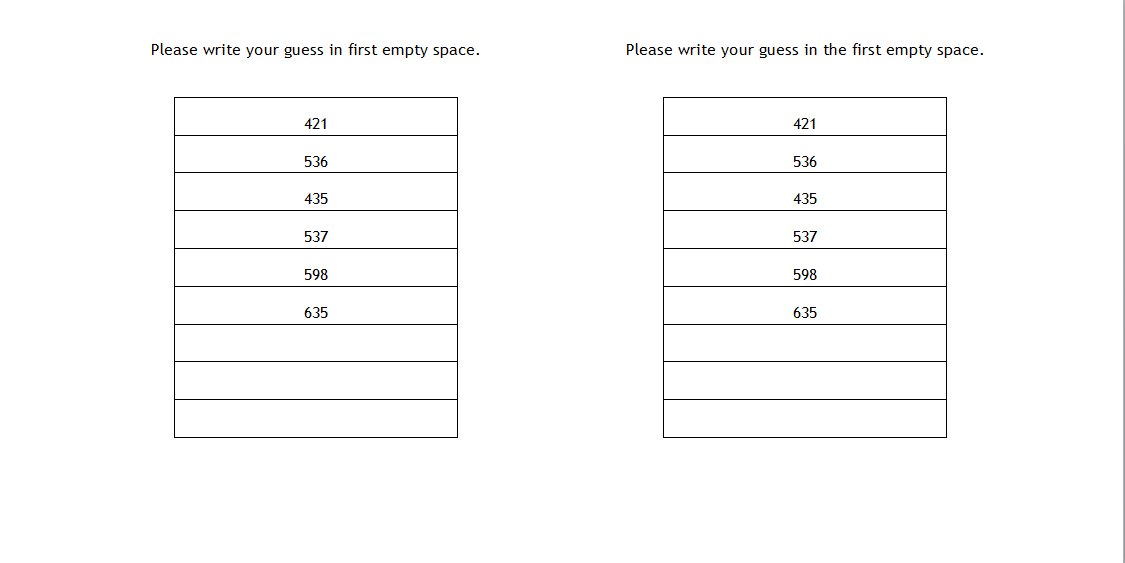
\includegraphics[width=\textwidth]{psych1}
\chapter{Blank guess sheets}
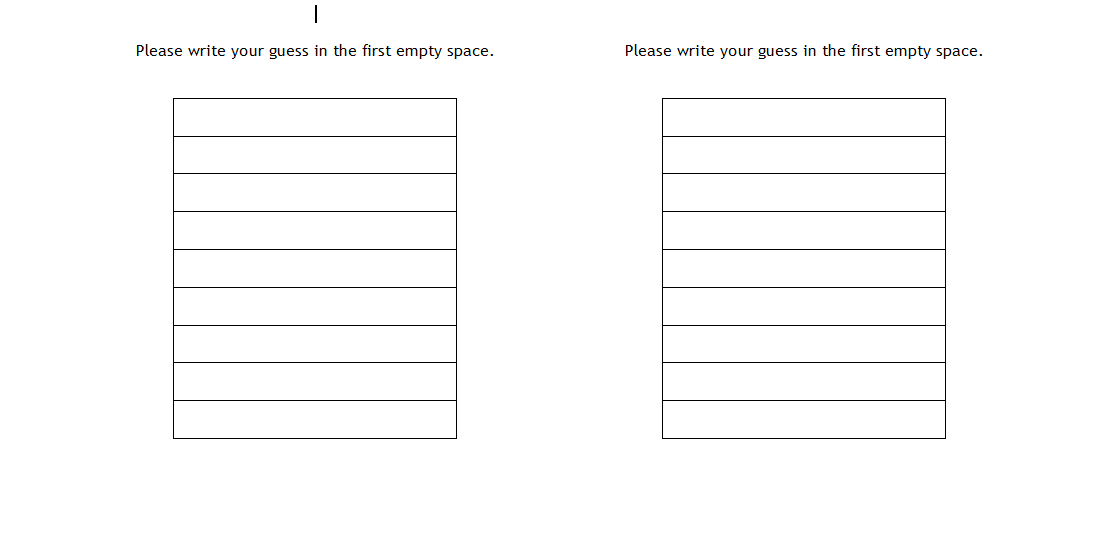
\includegraphics[width=\textwidth]{psych2}
\chapter{Raw results table}
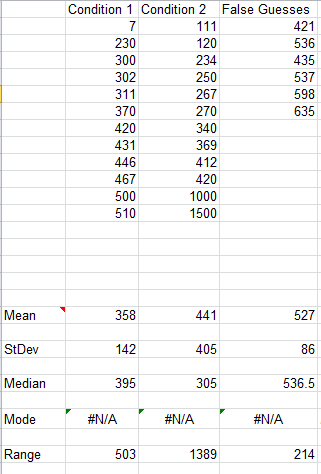
\includegraphics[width=\textwidth]{psych3}
\chapter{Informed consent document}
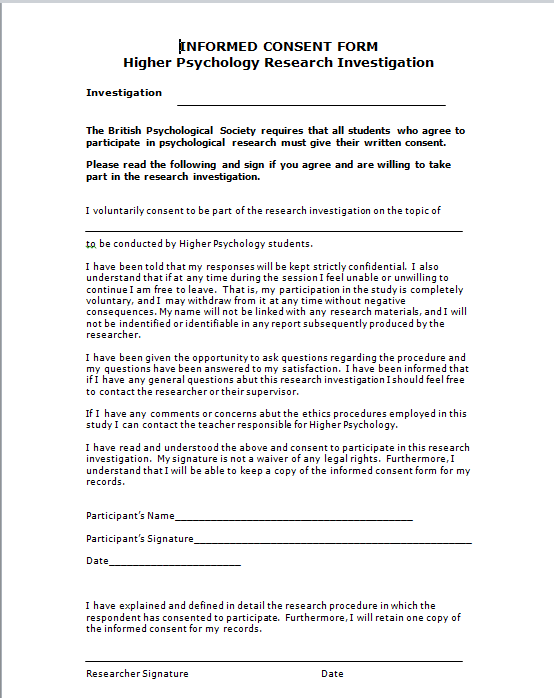
\includegraphics[width=\textwidth]{psych4}
\chapter{Information sheet for participants}
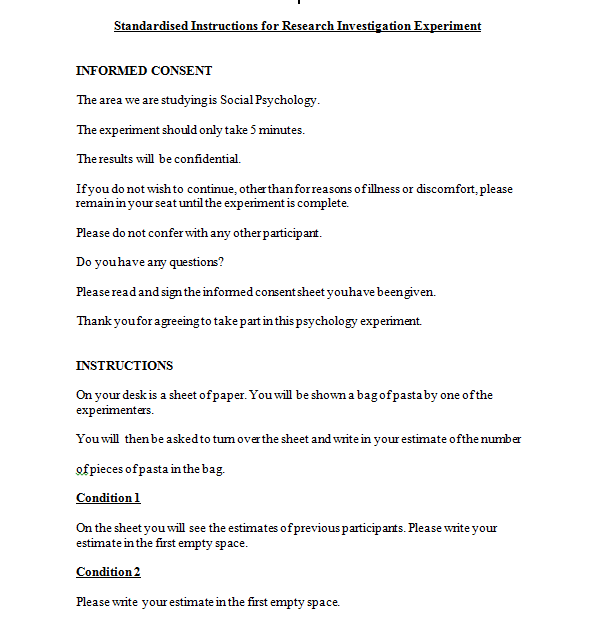
\includegraphics[width=\textwidth]{psych5}
\end{document}
